\documentclass[11pt,a4paper]{article}

% -------------------- Packages --------------------
\usepackage[a4paper,margin=1in]{geometry}
\usepackage{graphicx}
\usepackage{booktabs}
\usepackage{array}
\usepackage{tabularx}
\usepackage{multirow}
\usepackage{float}
\usepackage{amsmath}
\usepackage{microtype}
\usepackage[hidelinks]{hyperref}
\usepackage{xcolor}
\usepackage{enumitem}
\usepackage{caption}
\usepackage{subcaption}
\usepackage{fancyhdr}

% % -------------------- Page style --------------------
% \pagestyle{fancy}
% \fancyhf{}
% \lhead{CSE214 -- }
% \rhead{Apache JMeter}
% \cfoot{\thepage}

% -------------------- Replace these --------------------
\newcommand{\studentname}{Mehedi Hasan Kanon}
\newcommand{\studentid}{2305052}
\newcommand{\sectionname}{A2}
\newcommand{\videolink}{https://youtu.be/7qkEvcth1Rk?si=FfufbaZWguLESZgM}


% -------------------- Figure helper --------------------
% Put screenshots inside a folder named "figures/" next to this .tex file.
% If a file is missing, the report prints a placeholder box instead.
\newcommand{\reportfigure}[3][0.92\textwidth]{%
\begin{figure}[H]
    \centering
    \IfFileExists{#2}{%
        \includegraphics[width=#1]{#2}%
    }{%
        \fbox{%
        \begin{minipage}[c][4.5cm][c]{0.86\textwidth}
            \centering
            \textbf{IMAGE PLACEHOLDER}\\[6pt]
            Put the following screenshot here:\\[4pt]
            \texttt{\detokenize{#2}}\\[10pt]
            \emph{#3}
        \end{minipage}}
    }
    \caption{#3}
\end{figure}
}

\begin{document}

% =====================================================
% Title page
% =====================================================
\begin{titlepage}
    \centering
    \vspace*{1.2cm}

    {\Large \textbf{CSE214 -- Software Engineering Sessional}}\\[0.5cm]
    {\LARGE \textbf{Offline on Performance and Load Testing}}\\[0.4cm]
    {\large Report on LoadLab Performance}\\[1.5cm]

    \begin{tabular}{rl}
        \textbf{Student Name:} & \studentname\\
        \textbf{Student ID:} & \studentid\\
        \textbf{Section:} & \sectionname\\
    \end{tabular}

    \vfill

    \textbf{YouTube Video Demonstration: }\\
    \url{\videolink}

    \vfill
\end{titlepage}

% =====================================================
% Video link
% =====================================================
% \section*{Video Demonstration}
% \addcontentsline{toc}{section}{Video Demonstration}

% The complete workflow demonstration video link:

% \begin{center}
%     \url{\videolink}
% \end{center}

% \noindent
% The video demonstrates the JMeter test-plan structure, HTTP recording setup, execution of the 50-thread and 100-thread profiles, Duration Assertion behavior, result collection, and HTML dashboard generation.

% \tableofcontents
% \newpage

% =====================================================
% \section{Introduction}
% % =====================================================

% Performance testing is used to evaluate how a software system behaves when subjected to a controlled workload. Instead of verifying only functional correctness, a performance test measures properties such as response time, throughput, bandwidth usage, and failure rate under different levels of load.

% This experiment uses Apache JMeter to evaluate the LoadLab web application hosted at \texttt{103.94.135.91:8080}. Five HTTP endpoints with different workload characteristics were tested under two load profiles: 50 threads and 100 threads. A 100-second ramp-up period was used in both profiles so that the principal experimental difference was the configured number of JMeter users.

% The objectives of this experiment were to:

% \begin{itemize}[leftmargin=*]
%     \item configure and record HTTP requests using JMeter;
%     \item execute controlled load tests using 50 and 100 threads;
%     \item measure minimum, maximum, and average response times;
%     \item compare throughput and network reception/transmission rates;
%     \item apply a Duration Assertion and observe controlled pass/fail behavior;
%     \item export raw test results and generate JMeter HTML dashboard reports.
% \end{itemize}

% % =====================================================
% \section{Target Application and Endpoints}
% % =====================================================

% The test plan contains five target endpoints, selected to represent different types of server behavior.

% \begin{table}[H]
% \centering
% \caption{Target HTTP endpoints}
% \label{tab:endpoints}
% \begin{tabularx}{\textwidth}{>{\ttfamily}l l X}
% \toprule
% \textnormal{\textbf{Endpoint}} & \textbf{Method} & \textbf{Purpose} \\
% \midrule
% / & GET & Baseline page request with a small response body and low expected latency. \\
% /notices & GET & Dynamic request with a randomized delay, useful for observing latency variation. \\
% /courses & GET & CPU-intensive request whose processing cost is intended to become more noticeable under load. \\
% /login & POST & Form-urlencoded authentication request using session cookies and HTTP redirection. \\
% /api/download/256 & GET & High-throughput download endpoint used to observe data-reception rate. \\
% \bottomrule
% \end{tabularx}
% \end{table}

% The authentication request used the following form parameters:

% \begin{verbatim}
% username=student
% password=student123
% \end{verbatim}

% =====================================================
\section{JMeter Setup}
% =====================================================

\subsection{JMeter Test Plan}

\begin{figure}[H]
    \centering
    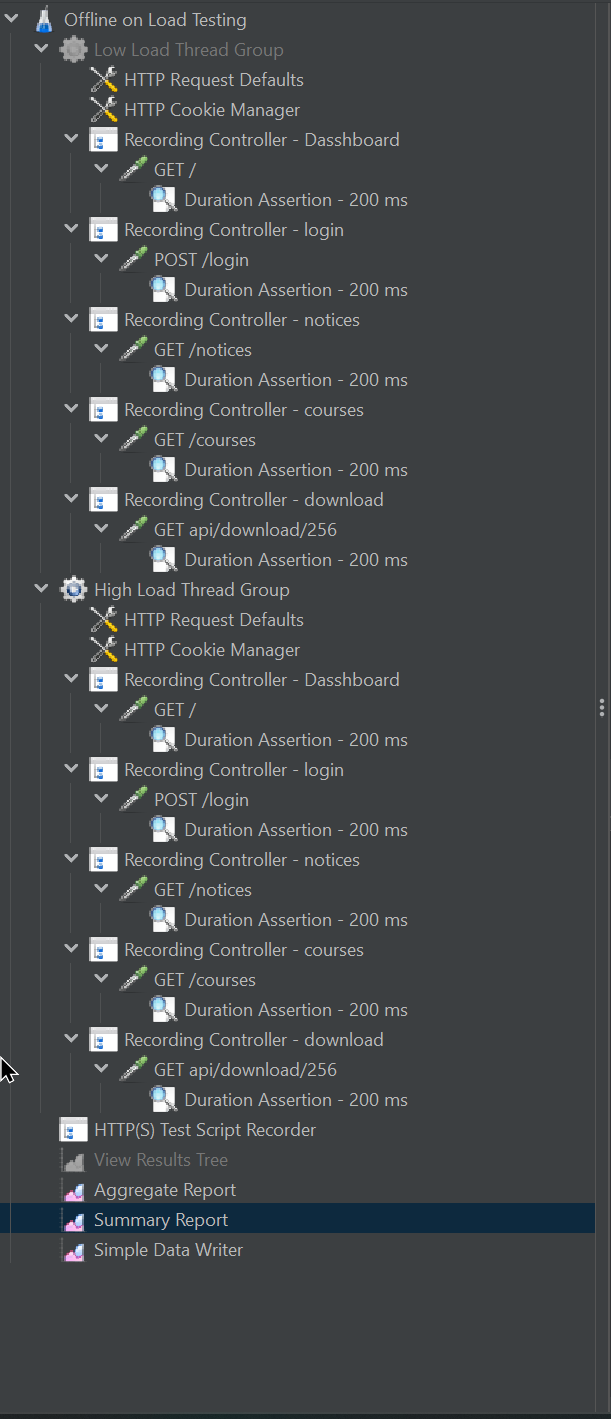
\includegraphics[width=0.92\textwidth,height=0.85\textheight,keepaspectratio]{figures/01-test-tree.png}
    \caption{Final JMeter test-plan tree containing high- and low-load profiles, Recording Controllers, Assertions, listeners, and an HTTP(S) Test Script Recorder.}
\end{figure}

\subsection{HTTP Request Defaults}

% The shared HTTP configuration was:

% \begin{table}[H]
% \centering
% \caption{HTTP Request Defaults}
% \begin{tabular}{ll}
% \toprule
% \textbf{Parameter} & \textbf{Value} \\
% \midrule
% Protocol & \texttt{http} \\
% Server name / IP & \texttt{103.94.135.91} \\
% Port & \texttt{8080} \\
% \bottomrule
% \end{tabular}
% \end{table}

\reportfigure{figures/04-http-defaults.png}
{HTTP Request Defaults configured for the LoadLab server.}

\subsection{Load Profiles}

% The two Thread Groups used identical request structure and a single iteration per thread.

% \begin{table}[H]
% \centering
% \caption{Load-profile configuration}
% \label{tab:loadprofiles}
% \begin{tabular}{lccc}
% \toprule
% \textbf{Profile} & \textbf{Threads} & \textbf{Ramp-Up} & \textbf{Loop Count} \\
% \midrule
% Low Load & 50 & 100 s & 1 \\
% High Load & 100 & 100 s & 1 \\
% \bottomrule
% \end{tabular}
% \end{table}

% With a 100-second ramp-up, the approximate thread-start rates were

% \[
% \frac{50}{100}=0.5 \text{ threads/s}
% \]

% for the low-load profile and

% \[
% \frac{100}{100}=1.0 \text{ thread/s}
% \]

% for the high-load profile.

% Thus, the experiment increases the request-arrival rate, but it does not represent 50 or 100 users becoming active simultaneously at one instant.

\begin{figure}[H]
\centering
\begin{subfigure}[t]{0.82\textwidth}
\centering
\IfFileExists{figures/02-thread-grp-50-config.png}{
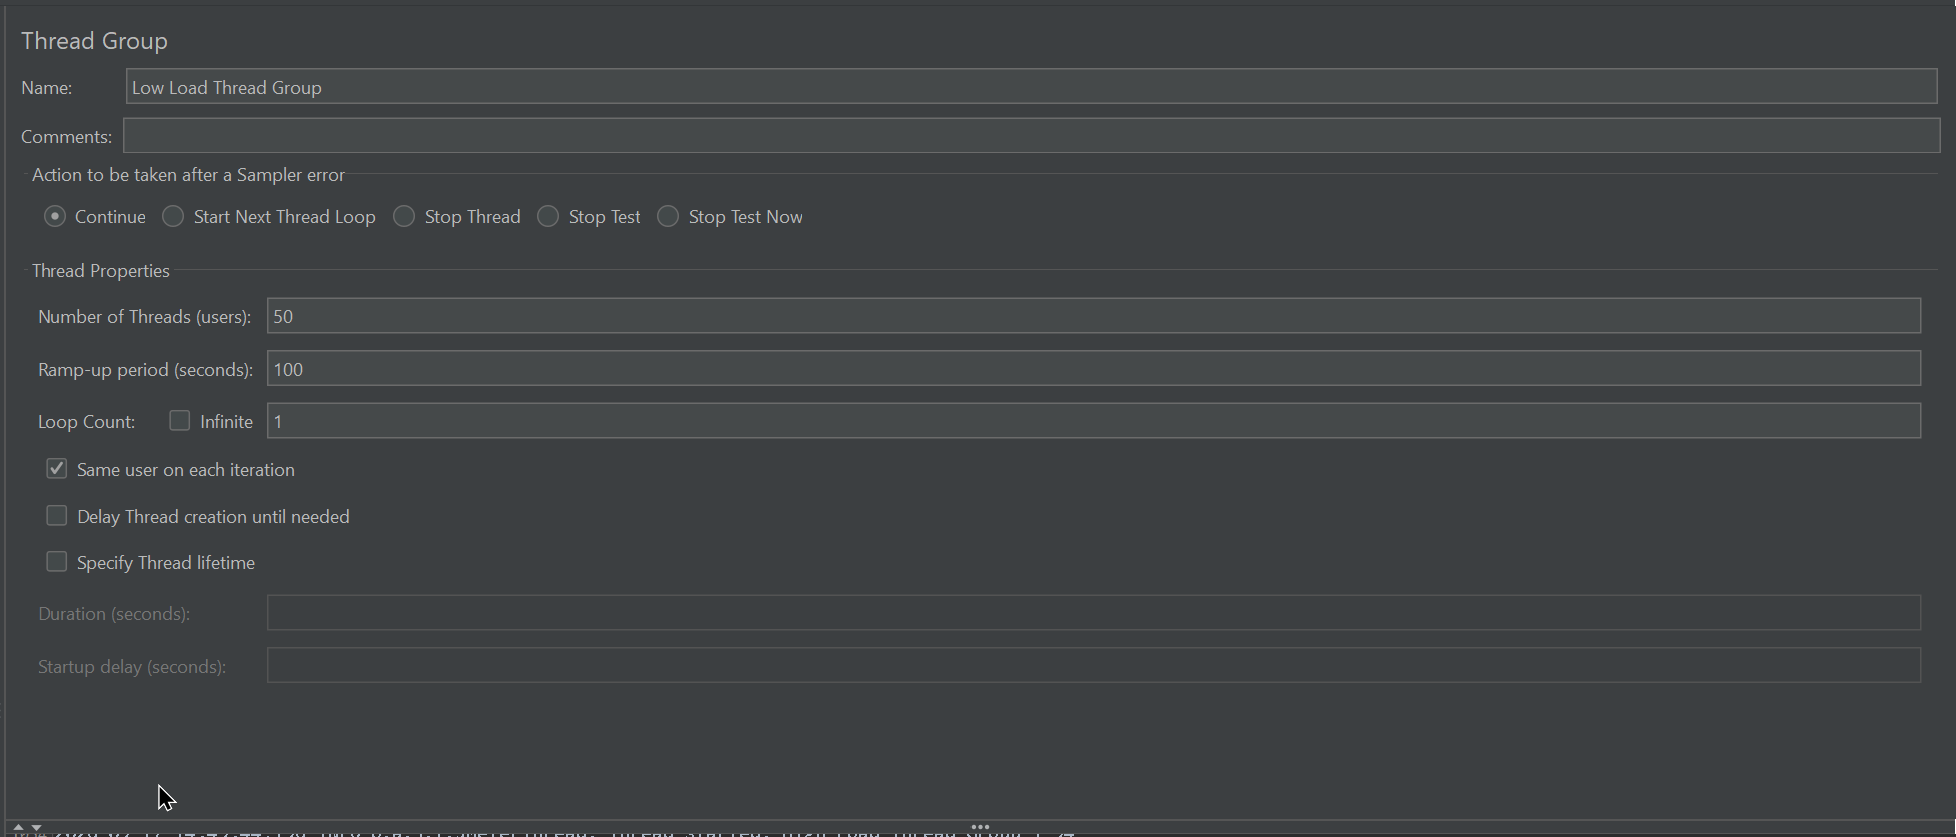
\includegraphics[width=\textwidth]{figures/02-thread-grp-50-config.png}
}{
\fbox{\parbox[c][4cm][c]{0.92\textwidth}{\centering
\textbf{IMAGE PLACEHOLDER}\\
\texttt{figures/02-thread-grp-50-config.png}\\
50-thread configuration}}
}
\caption{50-thread profile.}
\end{subfigure}
\hfill
\begin{subfigure}[t]{0.82\textwidth}
\centering
\IfFileExists{figures/03-thread-grp-100-config.png}{
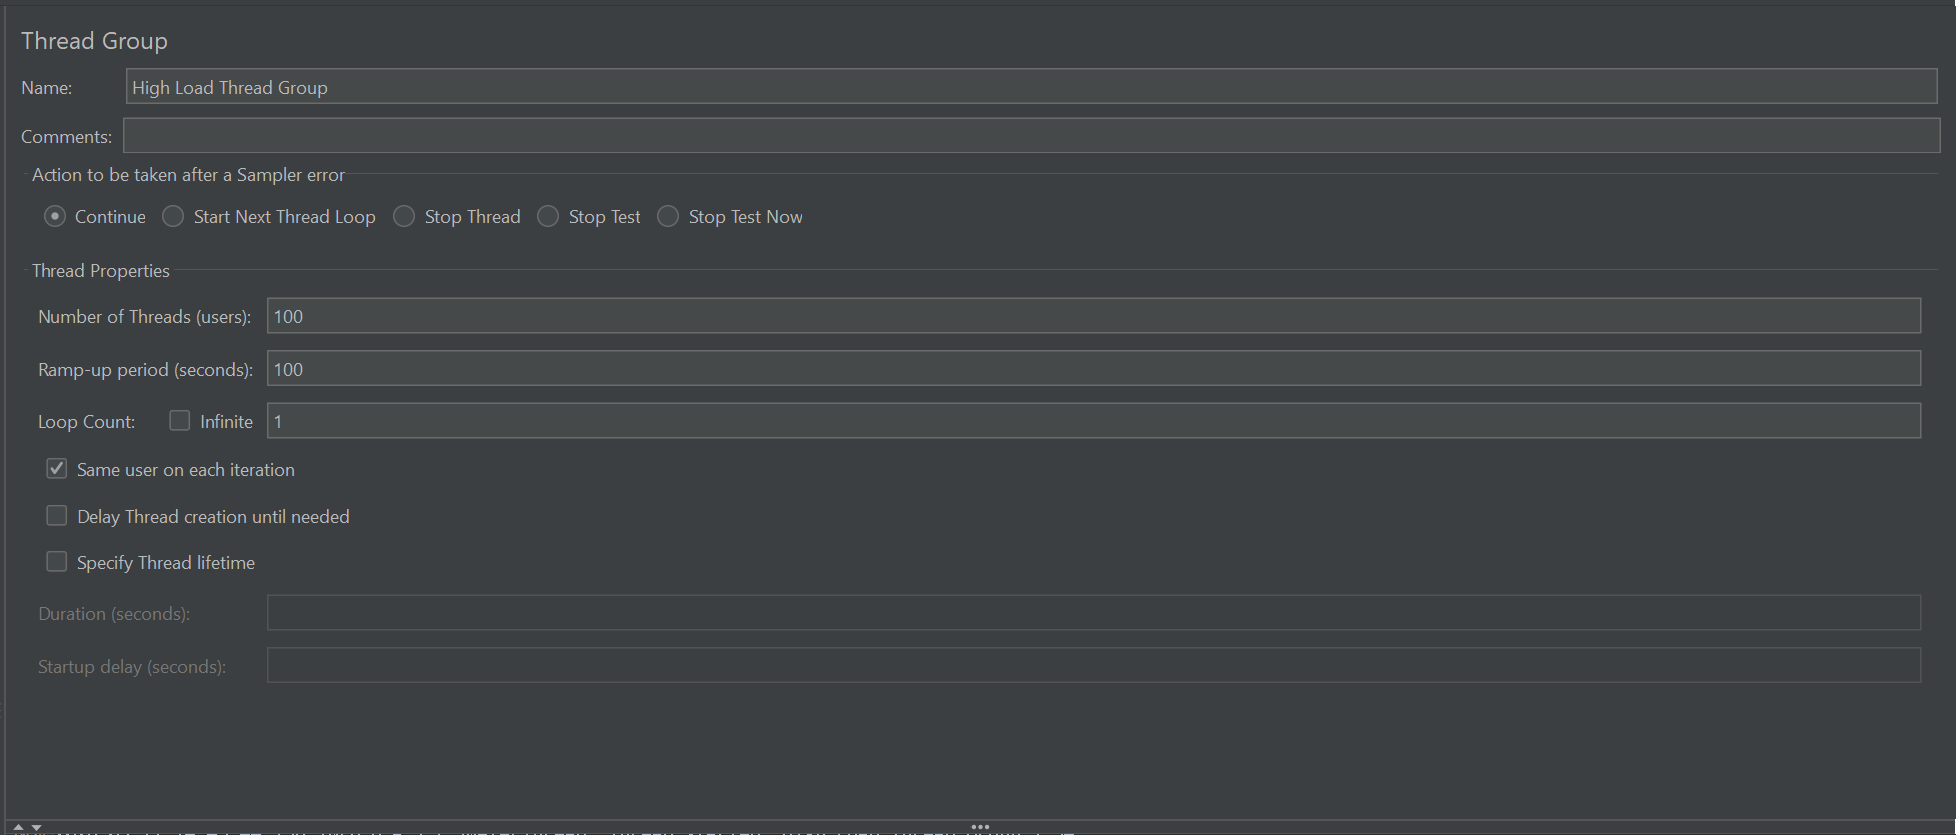
\includegraphics[width=\textwidth]{figures/03-thread-grp-100-config.png}
}{
\fbox{\parbox[c][4cm][c]{0.92\textwidth}{\centering
\textbf{IMAGE PLACEHOLDER}\\
\texttt{figures/03-thread-grp-100-config.png}\\
100-thread configuration}}
}
\caption{100-thread profile.}
\end{subfigure}
\caption{Thread Group configurations used for the two workload profiles.}
\end{figure}

\subsection{HTTP(S) Test Script Recorder}

The JMeter HTTP(S) Test Script Recorder was configured on local proxy port \texttt{8888}. Browser traffic was routed through the recorder via browser proxy settings. 

\reportfigure{figures/05-01-recorder-config.png}
{HTTP(S) Test Script Recorder configuration, including proxy port and target Recording Controller.}

\subsection{Authentication Request and Session Handling}

The login sampler used the POST method with the path \texttt{/login}. The username and password were configured as request parameters. Follow Redirects was enabled, allowing JMeter to process the authentication redirect chain. An HTTP Cookie Manager maintained session cookies separately for each JMeter thread.

\reportfigure{figures/06-login-params.png}
{POST \texttt{/login} sampler showing the username and password parameters.}

% =====================================================
\section{Duration Assertion}
% =====================================================

A Duration Assertion of

\[
T = 200 \text{ ms}
\]

\noindent was attached to each of the five main HTTP samplers. The assertion was configured for the main sample only.

% \noindent A sample satisfies the response-time requirement when

% \[
% t \leq 200\text{ ms},
% \]

% and fails the assertion when

% \[
% t > 200\text{ ms}.
% \]

\noindent The 200 ms value was suitable for this experiment because it produced both passing and failing requests.

\reportfigure{figures/07-duration-assert.png}
{Duration Assertion configured with a maximum permitted response time of 200 ms.}

\noindent An assertion failure does not necessarily indicate an HTTP transport or application failure.  A request may return HTTP 200 successfully but still be classified by JMeter as failed if its elapsed time exceeds 200 ms.

\reportfigure{figures/08-assertion-fail.png}
{Example of a request that returned a response but failed the 200 ms Duration Assertion.}

% =====================================================
% \section{Methodology}
% % =====================================================

% The experiment was carried out using the following procedure:

% \begin{enumerate}[leftmargin=*]
%     \item The five target interactions were recorded or configured as HTTP Request samplers.
%     \item Recorded browser noise and irrelevant static-resource requests were removed from the final test plan.
%     \item A one-user functional validation run was performed using View Results Tree.
%     \item The POST \texttt{/login} request was checked for the required credentials, redirect behavior, and session-cookie handling.
%     \item A 200 ms Duration Assertion was attached to each main HTTP request.
%     \item The 50-thread profile was enabled while the 100-thread profile was disabled.
%     \item Previous listener data was cleared and the 50-thread test was executed.
%     \item Raw sample results were written to a JMeter result file, and the Aggregate Report was exported.
%     \item The 50-thread HTML dashboard was generated from the raw JMeter results.
%     \item The procedure was repeated with the 100-thread profile enabled and the 50-thread profile disabled.
% \end{enumerate}

% View Results Tree was used for validation and visual inspection of assertion behavior rather than as the primary measurement source for the final comparison. The Aggregate Report was used for the required endpoint-level statistics.

% =====================================================
\section{Experimental Results}
% =====================================================

\subsection{Execution Time, Throughput, and Error Rate}

Table~\ref{tab:mainresults} presents the required minimum, maximum, average, throughput, and error-rate values for each endpoint.

\begin{table}[H]
\centering
\caption{Execution-time and throughput comparison}
\label{tab:mainresults}
\resizebox{\textwidth}{!}{
\begin{tabular}{lrrrrrr}
\toprule
\textbf{Endpoint} & \textbf{Threads} & \textbf{Min (ms)} & \textbf{Max (ms)} &
\textbf{Avg (ms)} & \textbf{Throughput (req/s)} & \textbf{Error \%} \\
\midrule
\texttt{GET /} & 50  & 19  & 107 & 41  & 0.51007 & 0 \\
\texttt{GET /} & 100 & 14  & 92  & 38  & 1.00983 & 0 \\
\midrule
\texttt{POST /login} & 50  & 90  & 404 & 162 & 0.50967 & 14 \\
\texttt{POST /login} & 100 & 74  & 751 & 140 & 1.00896 & 5 \\
\midrule
\texttt{GET /notices} & 50  & 114 & 412 & 266 & 0.50822 & 68 \\
\texttt{GET /notices} & 100 & 109 & 412 & 262 & 1.00871 & 72 \\
\midrule
\texttt{GET /courses} & 50  & 178 & 460 & 243 & 0.50816 & 84 \\
\texttt{GET /courses} & 100 & 168 & 298 & 233 & 1.00826 & 81 \\
\midrule
\texttt{GET /api/download/256} & 50  & 26 & 457 & 56 & 0.50901 & 4 \\
\texttt{GET /api/download/256} & 100 & 25 & 573 & 44 & 1.00958 & 1 \\
\bottomrule
\end{tabular}
}
\end{table}

\subsection{Bandwidth Comparison}

\begin{table}[H]
\centering
\caption{Throughput and network-rate comparison}
\label{tab:bandwidth}
\resizebox{\textwidth}{!}{
\begin{tabular}{lrrrr}
\toprule
\textbf{Endpoint} & \textbf{Threads} & \textbf{Throughput (req/s)} &
\textbf{Received (KB/s)} & \textbf{Sent (KB/s)} \\
\midrule
\texttt{GET /} & 50  & 0.51007 & 1.21 & 0.06 \\
\texttt{GET /} & 100 & 1.00983 & 2.40 & 0.12 \\
\midrule
\texttt{POST /login} & 50  & 0.50967 & 76.83 & 0.26 \\
\texttt{POST /login} & 100 & 1.00896 & 152.09 & 0.52 \\
\midrule
\texttt{GET /notices} & 50  & 0.50822 & 3.79 & 0.14 \\
\texttt{GET /notices} & 100 & 1.00871 & 7.52 & 0.27 \\
\midrule
\texttt{GET /courses} & 50  & 0.50816 & 22.10 & 0.14 \\
\texttt{GET /courses} & 100 & 1.00826 & 43.84 & 0.27 \\
\midrule
\texttt{GET /api/download/256} & 50  & 0.50901 & 130.45 & 0.14 \\
\texttt{GET /api/download/256} & 100 & 1.00958 & 258.73 & 0.28 \\
\bottomrule
\end{tabular}
}
\end{table}

The Aggregate Report totals were:

\begin{table}[H]
\centering
\caption{Overall aggregate metrics}
\label{tab:totals}
\begin{tabular}{lrrr}
\toprule
\textbf{Metric} & \textbf{50 Threads} & \textbf{100 Threads} & \textbf{Change} \\
\midrule
Average response time & 154 ms & 143 ms & $-7.14\%$ \\
Total throughput & 2.53011 req/s & 5.00791 req/s & $+97.93\%$ \\
Received rate & 232.94 KB/s & 461.06 KB/s & $+97.93\%$ \\
Sent rate & 0.73 KB/s & 1.44 KB/s & $+97.26\%$ \\
Error rate & 34.0\% & 31.8\% & $-2.2$ percentage points \\
\bottomrule
\end{tabular}
\end{table}

% =====================================================
\section{Performance Analysis}
% =====================================================

\subsection{Average Response-Time Comparison}

The change in average response time between the two profiles was computed using

\[
\%\Delta t =
\frac{t_{100}-t_{50}}{t_{50}}\times 100\%.
\]

\begin{table}[H]
\centering
\caption{Change in average response time}
\label{tab:responsechange}
\begin{tabular}{lrrr}
\toprule
\textbf{Endpoint} & \textbf{50 Threads} & \textbf{100 Threads} & \textbf{Change} \\
\midrule
\texttt{GET /} & 41 ms & 38 ms & $-7.32\%$ \\
\texttt{POST /login} & 162 ms & 140 ms & $-13.58\%$ \\
\texttt{GET /notices} & 266 ms & 262 ms & $-1.50\%$ \\
\texttt{GET /courses} & 243 ms & 233 ms & $-4.12\%$ \\
\texttt{GET /api/download/256} & 56 ms & 44 ms & $-21.43\%$ \\
\bottomrule
\end{tabular}
\end{table}

\noindent The 100-thread run did not produce higher average response time in this particular experiment. All five average values decreased slightly. \newline 

\noindent The two profiles used the same 100-second ramp-up and only one loop per thread, so the requests were introduced gradually rather than maintaining all configured threads under sustained simultaneous load. Run-to-run variation and uncontrolled activity on the shared class server may also have influenced the measurements. \newline 

\noindent Despite the lower averages, some worst-case values increased. The maximum login response time increased from 404 ms to 751 ms, while the maximum download response time increased from 457 ms to 573 ms. This demonstrates that average latency alone does not fully describe tail behavior.

% \subsection{Home Page}

% The baseline \texttt{GET /} endpoint was the fastest page-oriented request. Its average response time was 41 ms under the 50-thread profile and 38 ms under the 100-thread profile. No requests exceeded the 200 ms assertion threshold, producing a 0\% error rate in both runs.

% This stable result is consistent with the endpoint's role as a lightweight baseline request.

% \subsection{Notice Board}

% The notice-board endpoint produced average response times of 266 ms and 262 ms for the 50-thread and 100-thread profiles, respectively. Its assertion-based error rates were high: 68\% and 72\%.

% Because this endpoint is designed with a randomized delay of approximately 100--400 ms, substantial variation is expected even when the load profile remains unchanged. A 200 ms assertion threshold falls inside that delay range; therefore, many otherwise valid HTTP responses naturally violate the response-time requirement.

% \subsection{Course Catalogue}

% The \texttt{/courses} endpoint recorded averages of 243 ms and 233 ms. Its error rates were 84\% and 81\%, the highest among the tested endpoints.

% This endpoint is CPU-intensive and has a relatively high base response time. Consequently, a 200 ms Duration Assertion is deliberately strict for this request. Inspection of failed samples showed HTTP 200 responses that were classified as failures because their elapsed time exceeded the configured threshold.

% The present run did not show a higher average at 100 threads. Given the gradual ramp-up and the shared testing environment, this experiment should not be treated as a direct measurement of server CPU utilization.

% \subsection{User Authentication}

% The parent \texttt{POST /login} sampler averaged 162 ms for 50 threads and 140 ms for 100 threads. The corresponding error rates were 14\% and 5\%.

% The login flow uses HTTP redirection and session cookies. Because Follow Redirects was enabled, JMeter also recorded redirect sub-samples. These appear in the HTML dashboard as \texttt{POST /login-0} and \texttt{POST /login-1}. They are implementation details of the redirect chain and are not treated as separate target endpoints in the assignment comparison table.

% \subsection{Bandwidth Download}

% The \texttt{/api/download/256} endpoint achieved the largest data-reception rate of all tested requests. The received rate increased from 130.45 KB/s to 258.73 KB/s, an increase of approximately

% \[
% \frac{258.73-130.45}{130.45}\times100 \approx 98.3\%.
% \]

% This near-doubling is consistent with approximately twice as many requests being scheduled over the same 100-second ramp-up window. It should therefore be interpreted as aggregate workload throughput rather than as evidence that the physical network bandwidth of the server doubled.

% =====================================================
\section{Assertion and Error-Rate Analysis}
% =====================================================

The Duration Assertion was central to the observed JMeter error percentages. Table~\ref{tab:errorcomparison} compares the endpoint-level failure rates.

\begin{table}[H]
\centering
\caption{Duration-Assertion-related error-rate comparison}
\label{tab:errorcomparison}
\begin{tabular}{lrrr}
\toprule
\textbf{Endpoint} & \textbf{50 Threads} & \textbf{100 Threads} & \textbf{Difference} \\
\midrule
\texttt{GET /} & 0\% & 0\% & 0 pp \\
\texttt{POST /login} & 14\% & 5\% & $-9$ pp \\
\texttt{GET /notices} & 68\% & 72\% & $+4$ pp \\
\texttt{GET /courses} & 84\% & 81\% & $-3$ pp \\
\texttt{GET /api/download/256} & 4\% & 1\% & $-3$ pp \\
\bottomrule
\end{tabular}
\end{table}

\noindent A failed JMeter sample must not automatically be interpreted as an HTTP protocol failure. During inspection, samples were observed that returned HTTP 200 OK but failed because the Duration Assertion detected an elapsed time greater than 200 ms. 

\reportfigure{figures/09-assertion-pass-1.png}
{Example of a sample that completed within the assertion threshold.}

% =====================================================
\section{HTML Dashboard Reports}
% =====================================================

JMeter HTML dashboards were generated from the raw result logs for both load profiles.

\reportfigure{figures/12-html-050.png}
{Generated JMeter HTML dashboard for the 50-thread test.}

\reportfigure{figures/13-html-100.png}
{Generated JMeter HTML dashboard for the 100-thread test.}

% The HTML report includes additional redirect sub-samples for the login flow. Therefore, the dashboard total sample count is larger than the five-endpoint Aggregate Report total. For example, the 50-thread Aggregate Report contains \(5\times50=250\) main samples, while the dashboard also includes login redirect sub-samples. The assignment comparison tables in this report use only the five required parent endpoint labels.

% The APDEX section of the generated dashboard was not used as the primary evaluation criterion because its default tolerance/frustration thresholds are independent of the 200 ms Duration Assertion used in this experiment.

% % =====================================================
% \section{Limitations}
% % =====================================================

% Several limitations should be considered when interpreting the results:

% \begin{itemize}[leftmargin=*]
%     \item \textbf{Shared server environment.} The LoadLab instance was shared among students. External traffic generated by other users could influence response time, throughput, and queueing behavior.
%     \item \textbf{Gradual ramp-up.} A 100-second ramp-up means the configured users are introduced gradually. The experiment therefore does not represent an instantaneous burst of 50 or 100 simultaneous requests.
%     \item \textbf{Single official run per profile.} The reported values describe the selected 50-thread and 100-thread runs. Repeated independent runs would be necessary to quantify run-to-run variance statistically.
%     \item \textbf{Client-side measurement.} JMeter observes timings and traffic from the load generator. No server-side CPU, memory, disk, or network-interface utilization measurements were collected, so bottleneck causes cannot be confirmed directly.
%     \item \textbf{Assertion threshold.} The 200 ms threshold was intentionally selected to create both passes and failures. Consequently, Error \% should not be interpreted purely as application unavailability.
% \end{itemize}

% % =====================================================
% \section{Conclusion}
% % =====================================================

% A complete Apache JMeter load-testing workflow was configured and executed against five LoadLab endpoints using 50-thread and 100-thread profiles with a 100-second ramp-up.

% The 100-thread profile approximately doubled endpoint throughput from about 0.51 requests/s to about 1.01 requests/s. Overall received network rate increased from 232.94 KB/s to 461.06 KB/s. The dedicated download endpoint showed the highest reception rate, increasing from 130.45 KB/s to 258.73 KB/s.

% The average response times did not increase in the 100-thread run; instead, small decreases were observed. Given the gradual ramp-up, single-loop workload, run-to-run variability, and shared test environment, this result does not imply that increased load inherently improves response time.

% The 200 ms Duration Assertion successfully generated both passing and failing events. The homepage remained below the threshold in all samples, while the randomized notice-board request and CPU-intensive course request produced substantially higher assertion-failure rates. This demonstrated the difference between a successful HTTP response and a JMeter sample that fails a performance requirement.

% Overall, the experiment provided practical experience in HTTP request recording, load-profile design, response-time validation, throughput and bandwidth measurement, assertion-based performance criteria, raw-result export, and JMeter HTML dashboard generation.

\end{document}
